\chapter{Design}
\label{chapter:design}

The design phase focuses on developing hardware and software architecture, which addresses performance, security, and data structure \cite{Hausen}. Furthermore, alongside technical considerations, attention is given to the user interface, ensuring it is user-friendly and navigable \cite{Hausen}.

This section offers an overview of the project's software architecture, highlighting the utilization of the MVC model and integrating a thread pool to enhance efficiency. Moreover, it delves into user interface design principles, emphasizing familiarity and simplicity. The wireframe, color scheme, and font selection are also discussed. The concept of user flow is explained through task flows and Wireflow.

\section{Software Architecture}
\label{sec:software-architecture}

The design of the MVC architecture for this project is shown in Figure \ref{fig:architechture}. Within the figure, the separation between each MVC component is clearly shown. The view and the model components are completely decoupled from each other, and the controller component is responsible for mediating the interaction between the view and the model.

Another feature shown in Figure \ref{fig:architechture} is the implementation of multiple views and controllers. This implementation ensures the system's scalability, a crucial project requirement defined previously in Section \ref{section:project-requirements}. By doing so, the functionality within the project can easily be expanded in the future.

\begin{figure}[!ht]
    \centering
    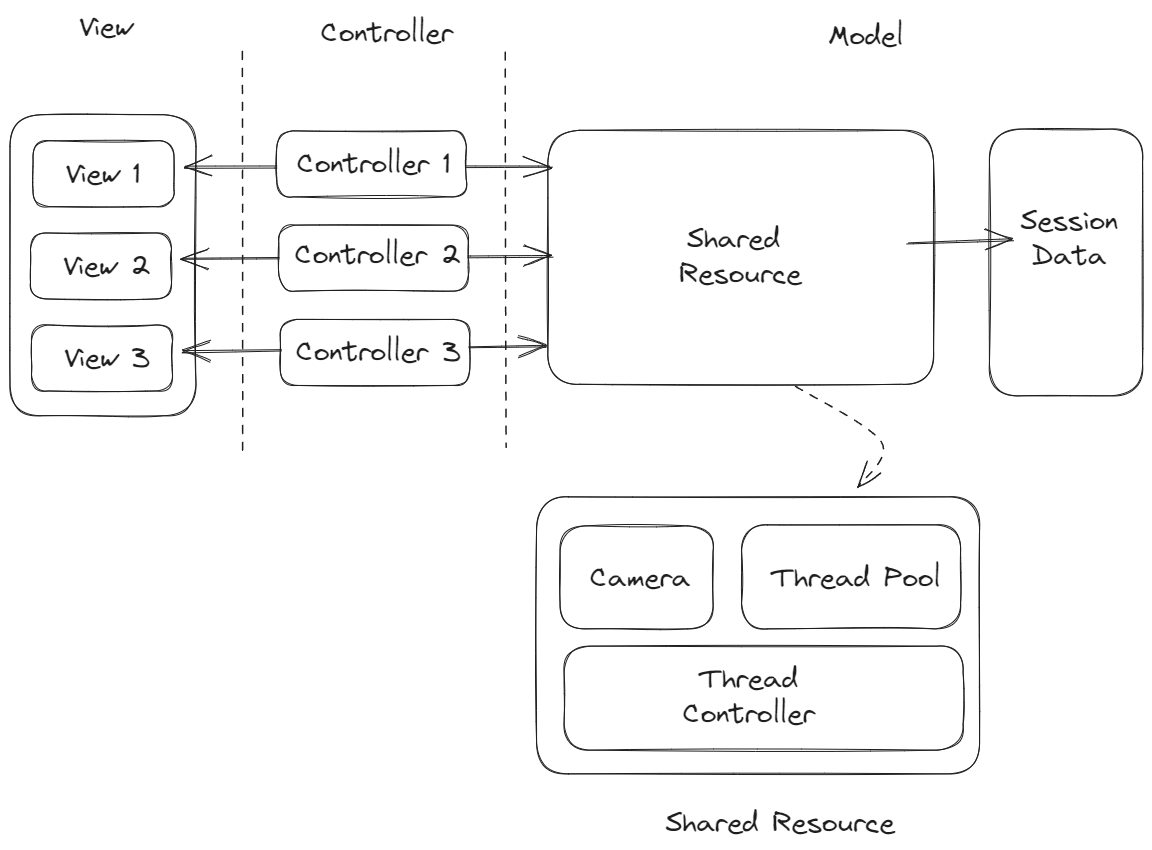
\includegraphics[width=0.8\textwidth]{texs/Part2/chapter3/image/architecture.png}
    \caption{Software Architecture}
    \label{fig:architechture}
\end{figure}

\begin{figure}[!ht]
    \centering
    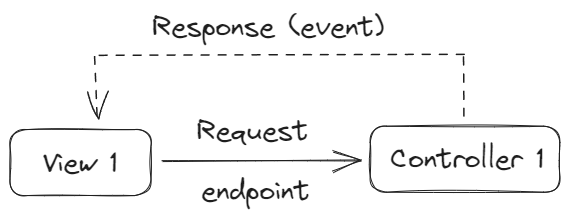
\includegraphics[width=0.6\textwidth]{texs/Part2/chapter3/image/reqres.png}
    \caption{Request-Response Cycle}
    \label{fig:reqres}
\end{figure}

Moreover, implementing multiple controllers is necessary to prevent the \textit{Promiscuous Controller} problem as mentioned in \cite[2127]{Aniche2017}. This issue occurs when a single controller handles too many responsibilities, causing it to become bloated and difficult to maintain. By separating the controllers, each controller can efficiently handle specific responsibilities, making the system easier to maintain.

It is worth noting that the view components are carefully separated from each other. This intentional separation prevents any accidental mixing of view elements. For instance, View 1 may require specific UI components, while View 2 may need an entirely different set. This implementation simplifies the implementation process and makes it easier to understand.

The design of request and response cycles is shown in Figure \ref{fig:reqres}. This design is crucial because it enables the View and Controller to communicate with each other. The Controller will handle any request from View via provided endpoints, process it, and then send it back to the View as a response via event.

The model components have two subcomponents: the Shared Resource and Session Data. Both subcomponents are responsible for managing the data within the application. In the later section, we will discuss the design of these subcomponents in detail.

\subsection{Thread Pool}
\label{subsec:thread-pool}

A thread pool is a collection of worker threads that efficiently execute asynchronous callbacks on behalf of the application \cite{Karl-Bridge-Microsoft}. It is primarily used to reduce the number of application threads and provide management of the worker threads \cite{Karl-Bridge-Microsoft}.

Utilizing a thread pool involves following some basic principles. Initially, a group of threads is created, called workers or executors. The number of threads in the pool is typically determined by the CPU's number of cores \cite{GeekforGeek_2020}. A more significant number of thread pools, meaning more parallel tasks, can be executed, resulting in a much better efficiency. However, a thread pool that's too large can result in resource inefficiencies, where precious time is expended in context switching between threads \cite{GeekforGeek_2020}.

Once the creation of workers is complete, they become available for execution. Tasks can be created and added to a queue. Any available workers will then be assigned to a task from the queue. Once a task is finished, the worker will receive a new task until the queue is empty. If all workers are currently busy, the task will wait in the queue until an available worker can be assigned to it. \cite{GeekforGeek_2020}

\begin{figure}[!ht]
    \centering
    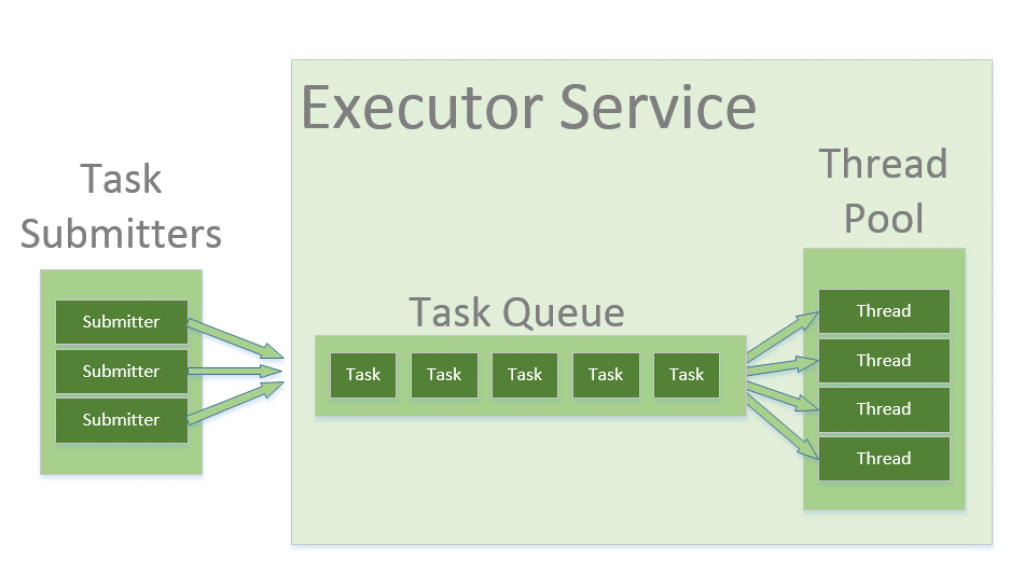
\includegraphics[width=0.65\textwidth]{texs/Part2/chapter1/image/threadpool.png}
    \caption{Thread Pool Architecture \cite{Paraschiv_2023}}
    \label{fig:thread-pool}
\end{figure}

Figure \ref{fig:thread-pool} shows the thread pool architecture overview. The thread pool object will improve the system's efficiency for this project. It is one of the required features for this project, as defined in Section \ref{section:project-requirements}. It solves one of the problems mentioned in \cite{Sabtu_2023}, where some computer vision algorithms are computationally expensive and can take a long time to execute.

Suppose the tasks are run in a single-threaded environment. In that case, the user has to wait for a long time until the task is completed, which is not ideal for a user interface application because it makes the application unresponsive. On the other hand, if multiple instances of the task are run in parallel without proper monitoring, the system may become overloaded, which can cause it to crash.

The thread pool implementation comes into play to solve this problem. It creates a fixed number of available threads, enabling parallelism while preventing the system from being overloaded. Additionally, the thread pool manages the threads, so the user does not have to worry about creating and managing them. The user only needs to create the task and submit it to the thread pool, which will assign the task to an available thread.

\subsection{Thread Controller}
\label{subsec:thread-controller}

Including a Thread Controller in the application is crucial because it effectively lightens the workload of the main controller, thus improving its efficiency and performance. By effectively managing complex threading tasks, the Thread Controller allows the main controller to focus solely on managing communications between the model and view.

Inside the Thread Controller, there are several groups of threads. It is important to note that these threads differ from those defined in a thread pool. In this context, the threads within the Thread Controller are specialized units responsible for executing specific business logic. Each thread operates independently, enabling the system to handle multiple tasks simultaneously.

Furthermore, the Thread Controller is designed with access to the thread pool. This integration empowers the system to carry out tasks that require parallel processing in an organized way. Tasks can be placed in a queue within the Thread Pool, ensuring they are executed efficiently and without resource conflicts.

The design of this system is focused on scalability. Developers can define groups of threads to customize the system to meet specific performance needs. Additionally, the Thread Controller allows developers to control thread execution from the controller closely. This design makes achieving a high level of customization and adaptability to varying workloads possible. This combination of the Thread Controller and thread pool creates a strong foundation for building responsive, efficient, and scalable applications.


\section{User Interface Design}
User Interface (UI) design is a crucial aspect of product development that focuses on a product's look, style, and interactivity \cite{Coursera_2023}. It is the first thing users encounter when they use an application or visit a website \cite{Coursera_2023}.
A user-friendly UI design is pivotal in enriching the user experience, boosting user engagement, and ultimately shaping the success of an application \cite{AlgoRepublic_2023}.

Various design guidelines can be used to create a user-friendly UI design. Paun \cite{Paun_2020} stated that familiarity with UI design benefits both users and designers. It streamlines workflows, ensures a seamless experience, and efficiently uses established conventions. Adhering to standards and maintaining consistency is essential for a unified and positive user experience.

Fleck \cite{Fleck_2021} argues that simplicity in design plays a crucial role in UI design. A simple design minimizes cognitive load and allows users to accomplish tasks efficiently. The author also emphasizes that it is essential to remember that simplicity does not mean sacrificing functionality; instead, it means prioritizing essential elements and removing any extraneous details that may cause confusion or overwhelm the user.

In GUI design, feedback is as important as consistency and simplicity. It comes in forms like visual cues and error messages, helping users understand the product's state and how to interact with it. This feedback lessens confusion, builds trust, and aids in learning how to use the product, even when errors occur. \cite{Florido_2022}

\subsection{Wireframe}
\label{subsec:wireframe}

A wireframe is a basic, simplified layout of a digital interface that outlines content placement and page components \cite{White_2023}. It is a quick way to present a concept or idea without extensive time or resources \cite{White_2023}.

Gupta \cite{Gupta_2023} stated that a good wireframe excludes elements that could divert attention from decisions about the application's structure. However, it instead prioritizes the functional purpose over visual aesthetics, presenting a straightforward, basic portrayal of the application's features in monochrome. The author also stated that designers should provide annotations to explain and elaborate on specific features, providing clarity and context.

Figure \ref{fig:wireframe} shows the rough sketch of the user interface that will be used for this project. The user interface will be divided into four main sections: the title panel, image panel, status panel, and button panel.


\begin{figure}[!ht]
    \centering
    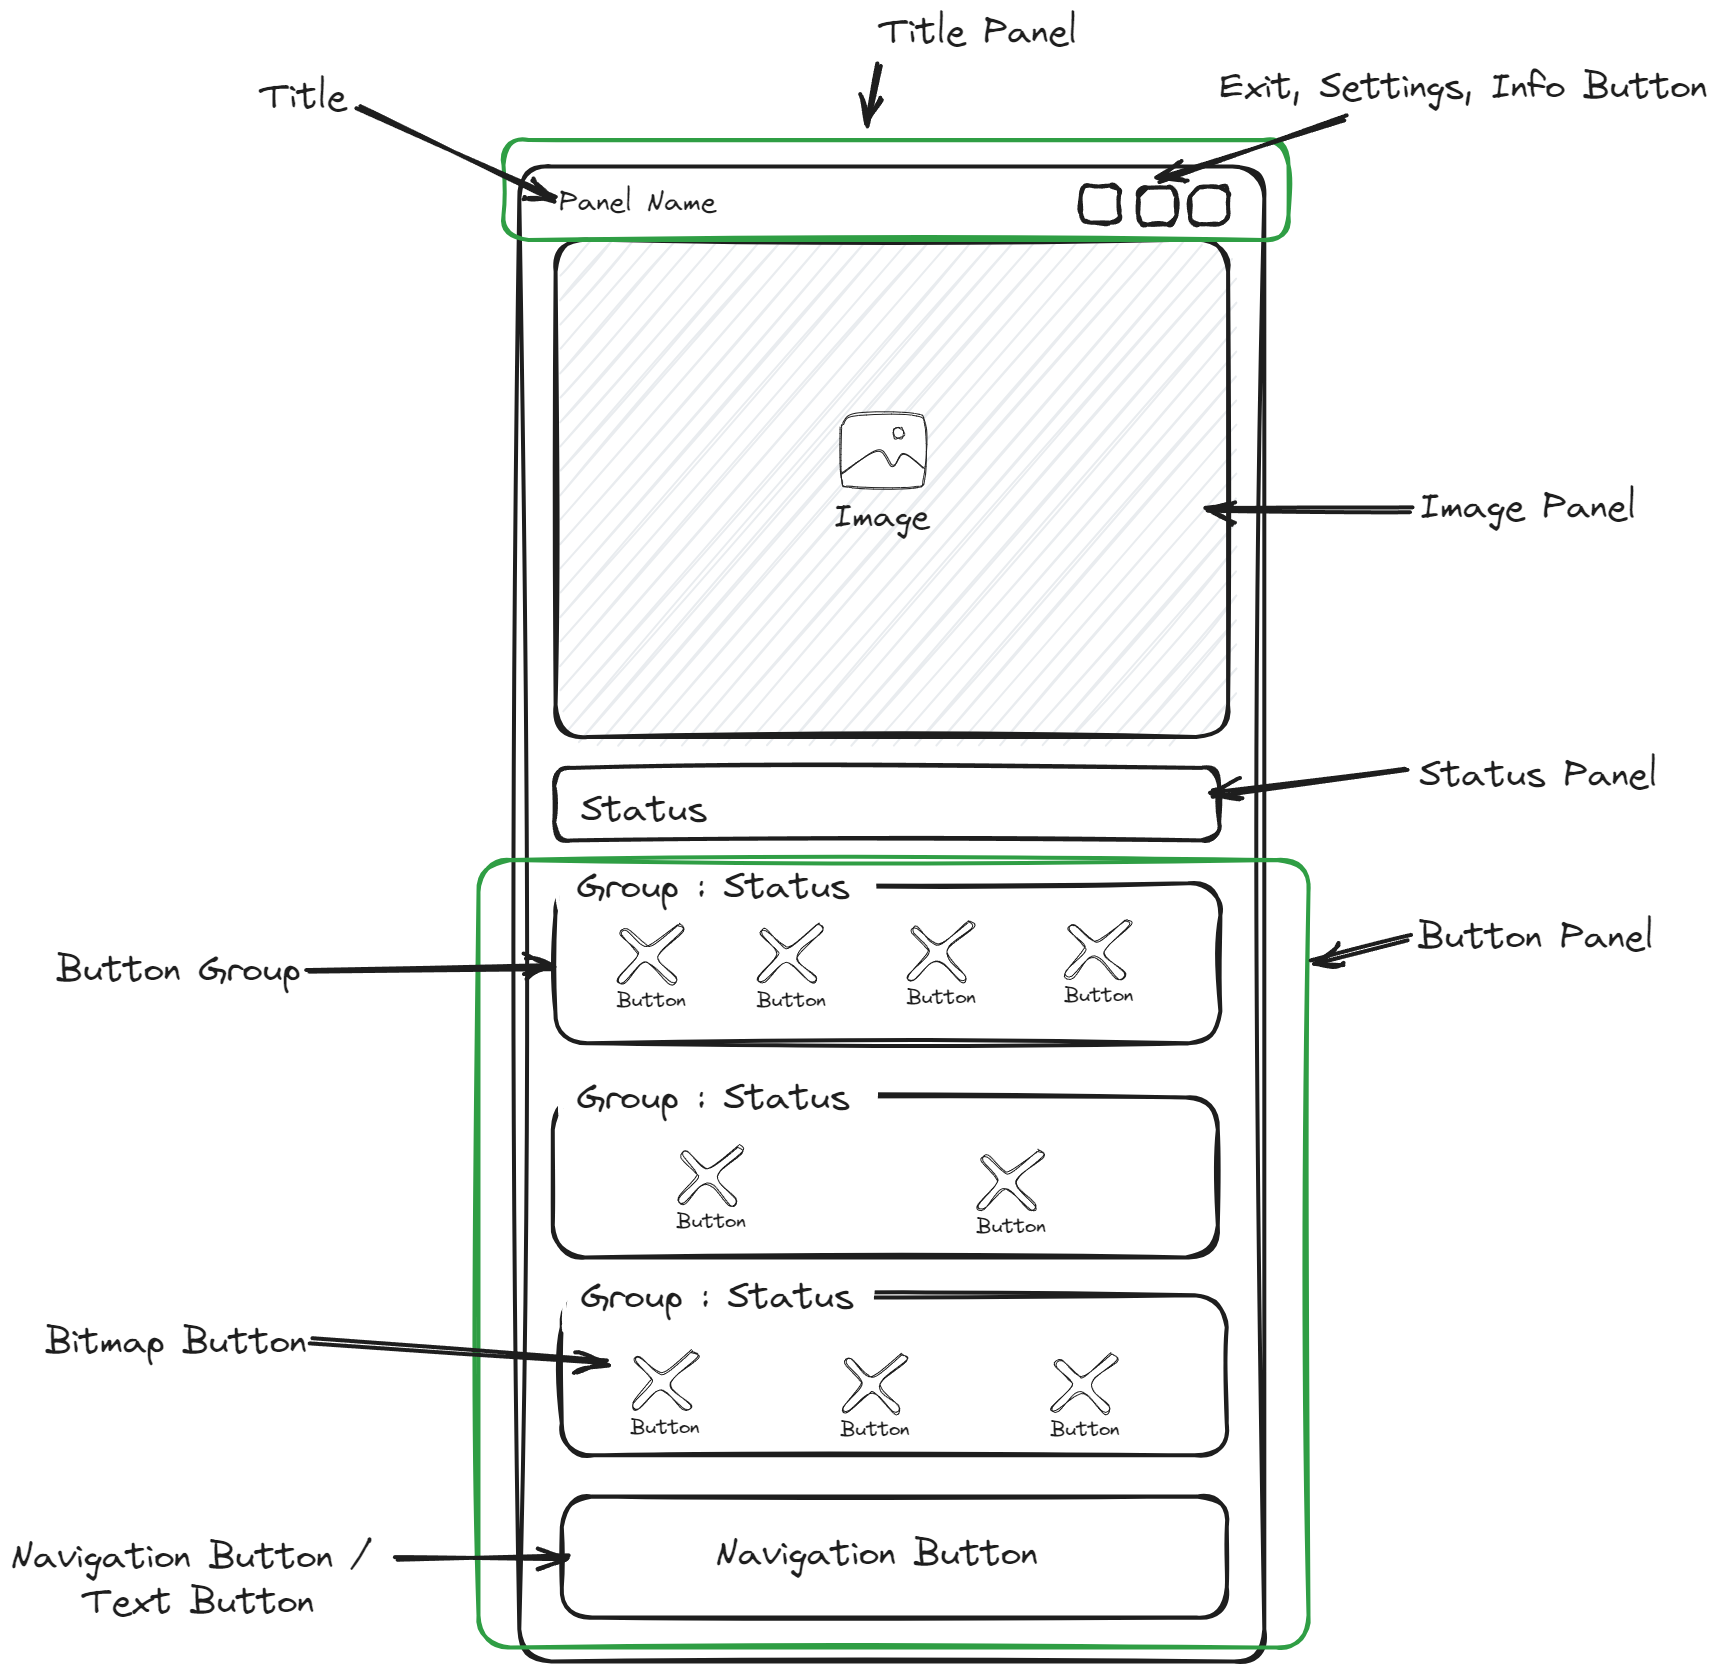
\includegraphics[width=0.65\textwidth]{texs/Part2/chapter3/image/wireframe.png}
    \caption{Wireframe}
    \label{fig:wireframe}
\end{figure}

The title panel plays a crucial role in the application by presenting the current panel and informing the user regarding the primary function of the panel. Additionally, this component provides various other features, such as closing the application, accessing the settings, and offering basic information about the application.

The image panel has the specific purpose of displaying images to the user. It is intended to display the images captured by the camera and the images being processed. The status panel, on the other hand, is intended to display the current status of the application to the user. Keeping the user informed about the application's status is crucial, allowing them to stay up-to-date with its progress.

The button panel will show the available buttons for the user to interact. The buttons will be categorized based on their functionality. There will be two kinds of buttons: bitmap buttons and text buttons.

\subsection{Color Scheme}

Color is a pivotal element in UI design, playing a vital role in evoking emotions, establishing hierarchy, and distinguishing design components \cite{M._2023}. With correct implementation, color can significantly improve the website or application's usability and overall user experience \cite{M._2023}.

Ou et al. \cite{Ou04} emphasized the strong correlation between color and emotion, highlighting how different colors evoke specific emotional responses. Their research underscores the significant impact that color choices can have on users' emotional experience.

Lewandowska and Olejnik-Krugly \cite{Lewandowska2021} stated that color is a significant aspect of visual communication. It plays a crucial role in conveying information. It is integral in identifying products, indicating quality, and influencing user interfaces.

They \cite{Lewandowska2021} also stated that colors can evoke diverse visual sensations, and their impact is often experienced in combination rather than in isolation, underscoring the crucial role of color in human perception and communication.

In their paper, Zhang and Ferris \cite{Zhang16} discuss essential factors to consider when choosing colors for design. These include the number of colors used, color harmony, and text overlay. Regarding the number of colors, designers have various options, such as using a single color with different shades or following the 60-30-10 rule for triadic color schemes, emphasizing primary, secondary, and accent colors. Figure \ref{fig:color-scheme} provides color combinations following the 60-30-10 rule.

\begin{figure}[!ht]
    \centering
    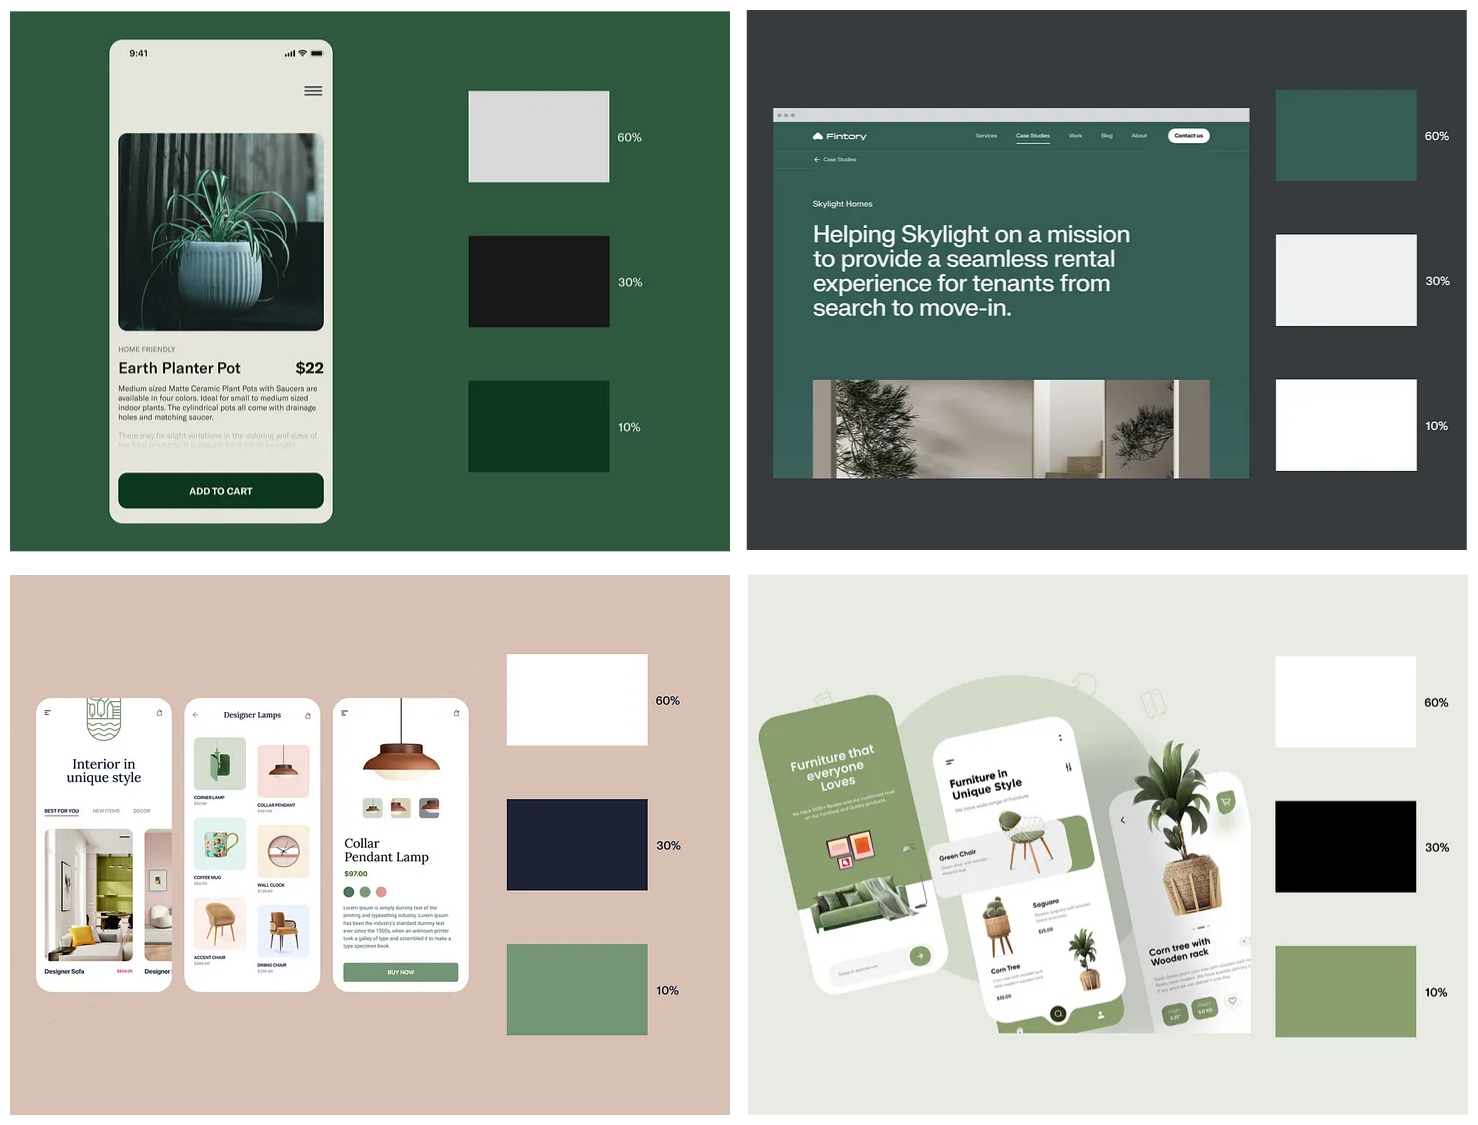
\includegraphics[width=0.8\textwidth]{texs/Part2/chapter3/image/colorexample.png}
    \caption{Example of Color Combination with 60-30-10 Rule \cite{M._2023}}
    \label{fig:color-scheme}
\end{figure}

In choosing the primary color, it is crucial to consider the brand's message and the emotions it wants to deliver \cite{M._2023}. The secondary color should complement the primary color and provide contrast to support the dominant color, while the accent color is used in features like buttons and pop-ups  \cite{M._2023}.

Figure \ref{fig:color-combination} shows the color combination used for this project. A simple white and black combination is used for the primary and secondary colors. Since the end-users will be the police officers, the blue shade is the accent color to represent the police force.

\begin{figure}[!ht]
    \centering
    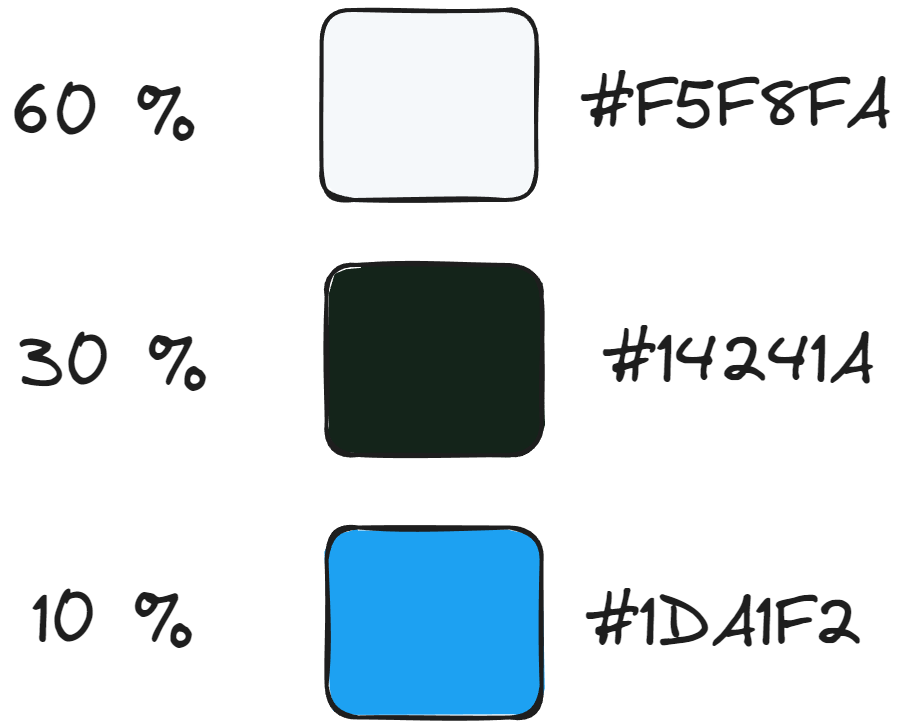
\includegraphics[width=0.45\textwidth]{texs/Part2/chapter3/image/colorcombination.png}
    \caption{Color Combination}
    \label{fig:color-combination}
\end{figure}

\subsection{Typography}Typography is critical in UI design, as over 90\% of online information is presented in text form \cite{Fitz-Patrick_2022}. It involves more than selecting attractive fonts; other factors such as typeface, font, character, baseline, and height are essential \cite{Fitz-Patrick_2022}.

Sawyer et al. \cite{Sawyer2020} stated that picking the right font is essential. It affects how things look and how easy they are to read. This finding is especially true for glances on screens. The authors also stated that recent studies found that different fonts can make a big difference in how easy things are to read in real-life situations.

The font used for this project is Roboto, a sans-serif typeface family created by Google as the system font for its mobile operating system Android \cite{Mott_2022}. According to Google, this font is designed to provide the best reading experience across different devices \cite{Mott_2022}. Figure \ref{fig:roboto} shows example text with the Roboto font on multiple styles.

\begin{figure}[!ht]
    \centering
    
\includegraphics[width=0.65\textwidth]{texs/Part2/chapter3/image/roboto.png}
    \caption{Roboto Font}
    \label{fig:roboto}
\end{figure}

\subsection{User Flow}
\label{subsec:user-flow}

User flow in UI design refers to a user's path to complete a specific task within an application or website. It includes each step, from the starting point to the endpoint with diagrams that display a user's complete path when using a product \cite{Browne_2023}. They help designers understand and anticipate the cognitive patterns of users in order to create products that enable a state of flow \cite{Browne_2023}.

Our project will involve utilizing two user flow types to illustrate user-system interactions. The first type is the task flow, which outlines a step-by-step process users must follow to accomplish a specific task \cite{Trigo_2023}. Task flows do not incorporate design elements and are typically described in natural language \cite{Trigo_2023}. They provide an overview of the primary actions users need to take to achieve a particular objective or endpoint \cite{Rahul_2022}.

The other type is Wireflow, a visual representation of the screens and interactions a user follows to complete specific tasks \cite{Trigo_2023}. It combines aspects of a basic wireframe, task flow, and flowchart to advanced screen flows that depict multiple navigation paths in one diagram \cite{Trigo_2023}. Arrows and annotations between wireframes are added on a single canvas to indicate user paths while using the product \cite{Angeles}.

Figure \ref{fig:task-flow} shows the task flow of the application, showing the task required, from start to finish, to successfully measure the speed of a moving object. The Wireflow of the application is shown in Figure \ref{fig:wireflow}, showing available panels that the user can navigate.

\begin{figure}[!ht]
    \centering
    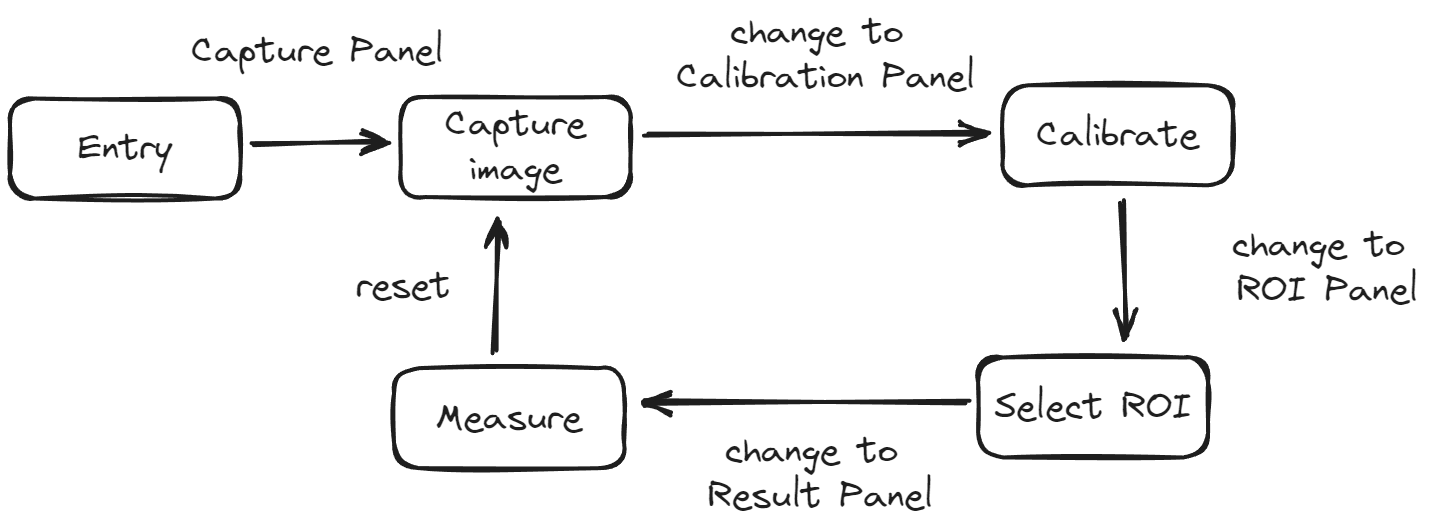
\includegraphics[width=0.8\textwidth]{texs/Part2/chapter3/image/taskflow.png}
    \caption{Task Flow}
    \label{fig:task-flow}
\end{figure}

\begin{figure}[!ht]
    \centering
    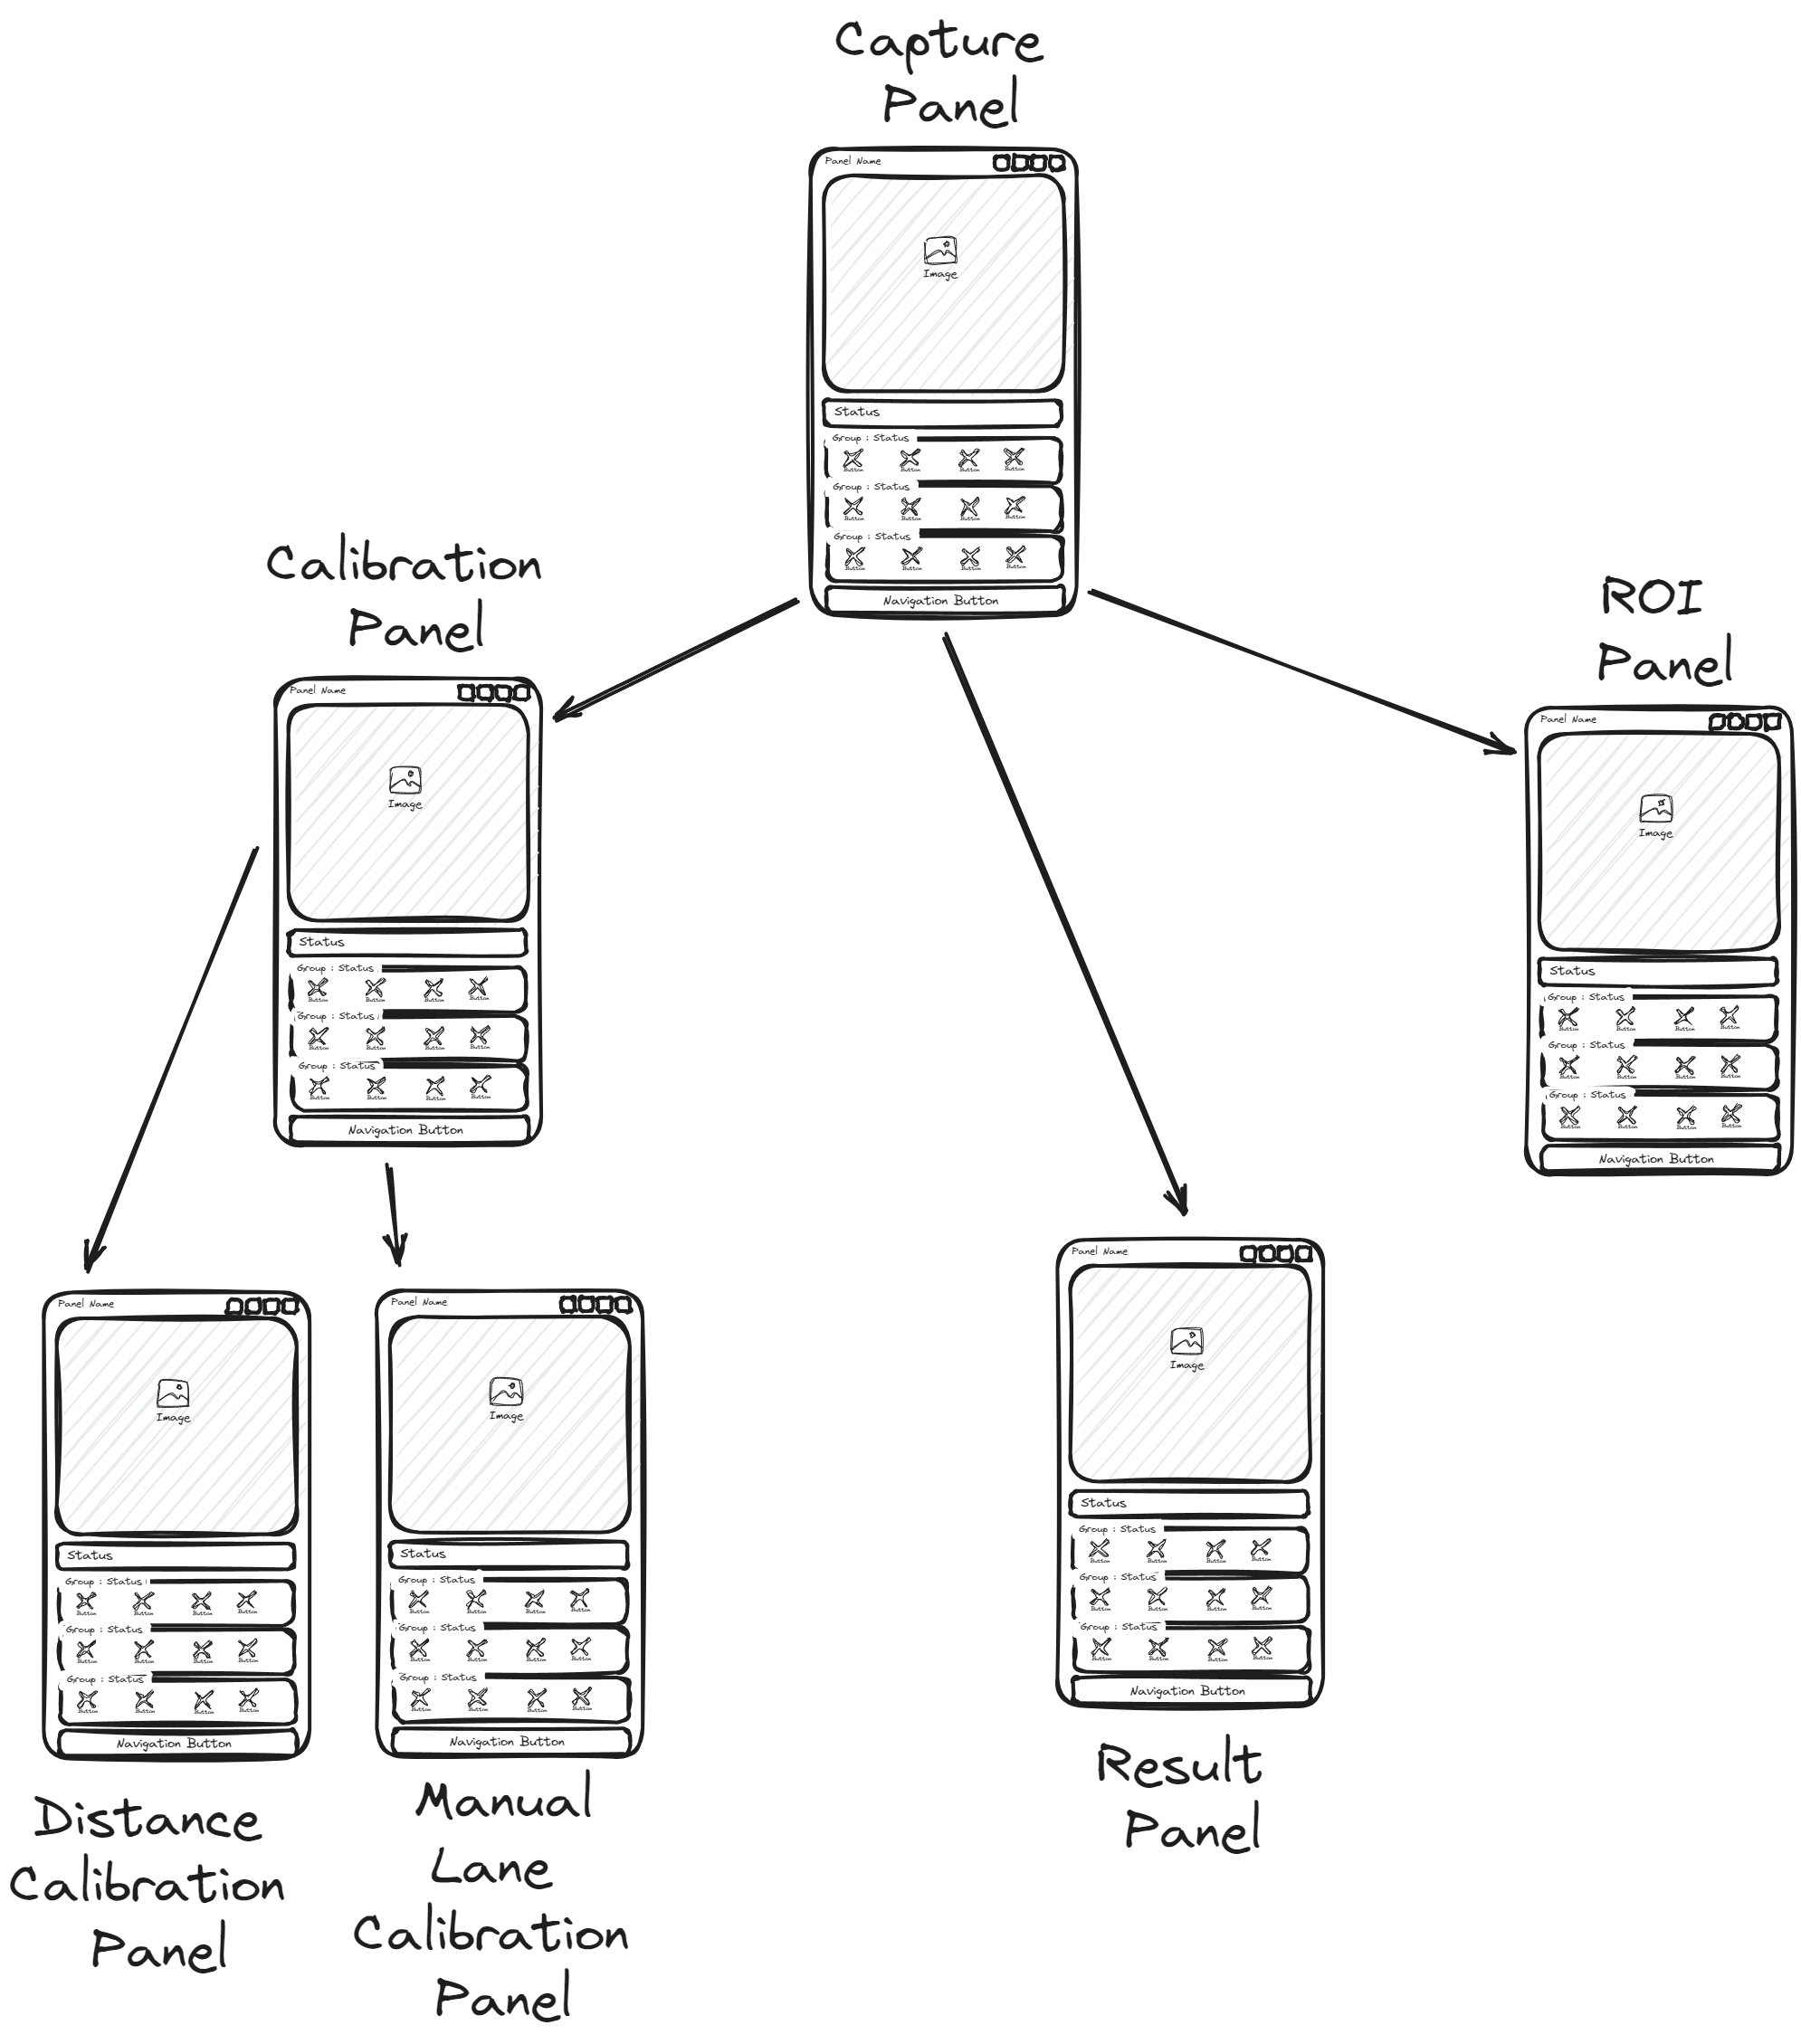
\includegraphics[width=0.8\textwidth]{texs/Part2/chapter3/image/wireflow.png}
    \caption{Wireflow}
    \label{fig:wireflow}
\end{figure}










